% ============================================================
% T-DOME Paper II: The Ego
% T-DOME three-paper series, Paper II
% ============================================================

\documentclass[12pt]{article}
\usepackage[margin=1in]{geometry}
\usepackage{amsmath,amssymb,amsthm}
\usepackage[hidelinks]{hyperref}
\usepackage{booktabs}
\usepackage{physics}
\usepackage{graphicx}
\usepackage{caption}
\usepackage{float}
\usepackage{array}
\newcolumntype{P}[1]{>{\raggedright\arraybackslash}p{#1}}
\graphicspath{{TDOME_II_supplement/}}

% Theorem environments — matching HAFF/Q-RAIF/T-DOME I style
\newtheorem{theorem}{Theorem}
\newtheorem{lemma}[theorem]{Lemma}
\newtheorem{proposition}[theorem]{Proposition}
\newtheorem{definition}[theorem]{Definition}
\newtheorem{remark}[theorem]{Remark}
\newtheorem{corollary}[theorem]{Corollary}
\newtheorem{conjecture}[theorem]{Conjecture}

\title{Spontaneous Symmetry Breaking of Reference Frames\\
as a Computational Cost Minimization Strategy}

\author{Sidong Liu, PhD \\
\small iBioStratix Ltd \\
\small \texttt{sidongliu@hotmail.com}}

\date{July 2026}

\begin{document}
\emergencystretch=2em
\raggedbottom
\hbadness=10000
\vbadness=10000
\maketitle

% ============================================================
\begin{abstract}
We investigate a conditional implementation model for bounded agents
that process memory-like state under finite computational resources.
Revised Paper~I~\cite{Liu2026TDOME_I} supplies a conditional
correlation-resource account; it does not establish universal memory
necessity, a universal Markovian ceiling, or a Landauer charge for
merely storing records.

The present paper therefore studies a declared raw $D$-channel archive
processed under a finite throughput budget.  Within that model,
symmetric processing of all declared channels can exceed the available
budget at a finite time, while a supplied coordinate selector can reduce
the declared load.  This is a conditional overload result for the stated
archive and algorithm, not a theorem that every persistent agent must
compress memory or break a symmetry.

Reference-frame selection is treated as a modelling strategy: a
privileged basis or coordinate projection packages a lower-dimensional
representation of the archive.  The rate-distortion calculation gives a
budget-dependent target dimension under the stated source, distortion,
and budget assumptions.  It does not prove that the ``self'' is a
universal survival-optimal structure.

The projected representation is accompanied by four diagnostic labels:
basis selection, frame drag, objective centering, and model
incompleteness.  Only basis selection follows from projection alone; the
other diagnostics require additional controller, update, objective, or
task assumptions.  A simple drift model gives a visibility crossover for
a fixed frame, motivating Paper~III's calibration problem without
establishing an undetectable universal Delusion Trap.
\end{abstract}

% ============================================================
\section{Introduction}
\label{sec:intro}

% ------------------------------------------------------------
\subsection{Context: The Problem of Overload}
\label{subsec:overload}

Revised Paper~I~\cite{Liu2026TDOME_I} gives an ELV-type
accounting identity in which initial correlations can fund a later
interval and proves a ceiling only for a fixed-Hamiltonian autonomous
Davies baseline.  It retracts both universal memory necessity and a
Landauer charge for merely storing or maintaining records.

The present paper therefore begins with an independent implementation
model: a raw, uncompressed $D$-channel archive processed under a finite
throughput budget.  Its overload is conditional on that archive and
algorithm.  The question is when a supplied coordinate selector can
reduce this declared load, not whether every persistent agent must
compress or break symmetry.

% ------------------------------------------------------------
\subsection{Position within the Series}
\label{subsec:series_position}

This paper is the second of three constituting the
\textbf{T-DOME} (Thermodynamic Dynamics of Observer-Memory
Entanglement) framework, the third pillar of a three-paper
program.

\begin{center}
\small
\setlength{\tabcolsep}{4pt}%
\begin{tabular}{@{}lP{3.2cm}cP{3.4cm}c@{}}
\toprule
\textbf{Framework} & \textbf{Question} & & \textbf{Result}
  & \textbf{Status} \\
\midrule
HAFF~\cite{Liu2026HAFF_A,Liu2026HAFF_B}
  & How does geometry emerge?
  & Ocean
  & Conditional algebra/dictionary models
  & Revised \\[3pt]
Q-RAIF~\cite{Liu2026QRAIF_A,Liu2026QRAIF_B}
  & What algebra must an observer have?
  & Fish
  & Clifford representation as model input
  & Revised \\[3pt]
T-DOME~I~\cite{Liu2026TDOME_I}
  & What can inter-epoch correlations fund?
  & Seed
  & Restricted baseline; accounting identity
  & Conditional \\[3pt]
\textbf{T-DOME~II} (this work)
  & When can a model select a frame?
  & Ego
  & Conditional coordinate selection
  & \textbf{This paper} \\[3pt]
T-DOME~III
  & When can residual statistics track drift?
  & Loop
  & Conditional Fisher calibration
  & Companion \\
\bottomrule
\end{tabular}
\end{center}

The three T-DOME papers form a conditional modelling sequence rather
than an irreversible theorem chain:
\begin{enumerate}
\item \textbf{Paper~I (The Seed):} An ELV-type balance identifies
  initial correlations as one possible interval resource.  Raw-archive
  overload is an implementation scenario, not a thermodynamic
  necessity.
\item \textbf{Paper~II (The Ego, this work):} Unbounded memory
  under finite computational resources causes processing
  overload in the coordinate-processing model.  This paper studies
  conditional feature selection; it does not prove universal SSB.
\item \textbf{Paper~III (The Loop):} Uncorrected bias diverges
  from a changing environment. A self-referential calibration
  loop (monitoring one's own prediction error) resolves the
  bias but requires the system to ``observe its own
  observation''---closing the self-calibration loop.
\end{enumerate}

% ------------------------------------------------------------
\subsection{Relation to Q-RAIF}
\label{subsec:qraif}

Revised Q-RAIF Papers A and B~\cite{Liu2026QRAIF_A,Liu2026QRAIF_B}
use a Clifford algebra $Cl(V,q)$ as a supplied representation choice;
persistence does not select it.  Paper C~\cite{Liu2026QRAIF_C} proves
only that the image of a separately supplied homomorphism lies in the
external algebra.  This paper adopts both the Clifford coordinates and
the representation map as model inputs.

The Clifford algebra $Cl(V,q)$, however, admits a non-trivial
\emph{automorphism group} $G = \mathrm{Aut}(Cl(V,q))$.
In the absence of external constraints, all elements of $G$
yield physically equivalent representations---the choice of
basis within the algebra is a \emph{gauge freedom}.
This gauge freedom is the mathematical substrate of the
symmetry considered in the conditional breaking analysis below.

The ``ego'' names a selected computational frame in that supplied
representation.  Whether a concrete optimum is a genuine gauge fixing
is a model condition, not an inherited theorem.

% ------------------------------------------------------------
\subsection{Relation to HAFF Paper~G}
\label{subsec:haff_g}

Revised HAFF Paper~G~\cite{Liu2026HAFF_G} offers
philosophy-of-science motivation and no fixed-point no-go theorem.  It
does not imply basis selection here.  Any connection between its
meta-level concern and this finite-budget model is motivation only.

% ------------------------------------------------------------
\subsection{Scope and Disclaimers}
\label{subsec:scope}

To prevent interpretational overreach, we state at the
outset what this paper does \emph{not} claim:
\begin{enumerate}
\item We do not claim that symmetry breaking is
  \emph{sufficient} for persistence.
  Paper~III addresses the additional requirements.
\item We do not claim that basis selection or spontaneous symmetry
  breaking is necessary for every bounded agent.  The results concern
  a declared coordinate-retention model.
\item The term ``ego'' or ``self'' is used in the
  control-theoretic sense: a fixed reference frame within
  the agent's internal algebra. It carries no implication
  of consciousness or subjective experience.
\item A broader structural analogy with classical philosophical
  concepts of selfhood exists but is outside the scope of
  this paper.
\end{enumerate}

\paragraph{Related work.}
The idea that bounded agents must compress their
representations has roots in Simon's bounded
rationality~\cite{Simon1955}, Shannon's
rate-distortion theory~\cite{Shannon1959,CoverThomas2006},
and Sims's rational inattention~\cite{Sims2003}, which
models finite-capacity decision-makers as solving a
rate-distortion problem---precisely the economic
counterpart of our $\mathcal{C}_{\mathrm{budget}}$
formalism.
The information bottleneck~\cite{Tishby2000}
formalises relevance-weighted compression and has been
applied to neural coding and deep
learning.
The role of decoherence in selecting preferred bases
(pointer states) is well established via quantum
Darwinism~\cite{Zurek2009}; here it motivates one
model-specific coordinate-selection rule.
Measures of non-Markovianity and their thermodynamic
consequences are reviewed
in~\cite{RivasHuelgaPlenio2014,BreuerPetruccione2002};
the connection to survival was established in Paper~I.

\paragraph{Summary of contributions.}
This paper separates three levels of result:
\begin{enumerate}
\item \textbf{Raw-channel load scaling law}
  a conditional accounting identity for a raw $D$-channel archive.
\item \textbf{Survival-weighted rate-distortion bound}
  a compactness-based existence result; the budget supplies only a
  capacity $k_{\max}$, not a universal optimal retained dimension.
\item \textbf{Delusion dynamics}
  a linear-drift visibility crossover plus an explicit two-mode
  example showing when gradient anti-correlation can occur.
\end{enumerate}

\paragraph{Result-status ledger.}
The original Computational Ceiling and SSB-necessity chain is retracted
(`TD-II-T3.5`).  Raw-channel load is an FD/I accounting proposition;
compression existence is conditional on a compact feasible model; SSB
is a model interpretation.  The Delusion Trap is downgraded
(`TD-II-T6.7`): visibility crossover is exact in the declared two-mode
geometry, while gradient sign and self-detection require extra dynamics.

% ============================================================
\section{Mathematical Preliminaries}
\label{sec:prelim}

% ------------------------------------------------------------
\subsection{Inherited Framework from Paper~I}
\label{subsec:inherited}

We briefly recall the key objects from
Paper~I~\cite{Liu2026TDOME_I} that the present work builds
upon.  The reader is referred to Paper~I for full definitions
and proofs.

\paragraph{Survival functional.}
For an open quantum system $S$ coupled to an environment $E$
at inverse temperature $\beta$, with dynamics $\Lambda$ and
external control protocol $H_{\mathrm{ctrl}}(t)$, the
survival functional is
\begin{equation}
\label{eq:survival_recall}
\mathcal{S}[\Lambda, \tau]
:= \Delta F - W[0,\tau],
\end{equation}
where $\Delta F = F(\rho(\tau)) - F(\rho(0))$ is the change
in non-equilibrium free energy and
$W = \int_0^\tau \tr(\rho(t)\,\dot{H}_{\mathrm{ctrl}}(t))\,dt$
is the work performed by the external protocol.

\paragraph{Restricted autonomous baseline.}
For a fixed-Hamiltonian Davies semigroup with no control, Paper~I proves
\begin{equation}
\label{eq:ceiling_recall}
\mathcal{S}[\Lambda^{\mathrm{M}}, \tau] \leq 0
\qquad\text{for all } \tau \geq 0.
\end{equation}
It does not extend this result to driven Markovian agents.

\paragraph{Non-Markovian advantage identity.}
For arbitrary initial states:
\begin{equation}
\label{eq:advantage_recall}
\beta\,\mathcal{S}
= -\Delta I(S{:}E)
  - \Delta D_{\mathrm{KL}}(\rho_E \| \rho_E^{\mathrm{th}})
  - \beta\,\Delta\langle H_{\mathrm{ctrl}} \rangle
  - \beta\,\Delta\langle H_{\mathrm{int}} \rangle.
\end{equation}

\paragraph{Conditional raw-archive model.}
Paper~I retracts a universal Landauer maintenance bound.  This paper
independently posits an uncompressed record stream.  Let $h_\mu$ be its
\emph{per-component} entropy rate~\cite{CrutchfieldYoung1989},
defined by
\begin{equation}
\label{eq:entropy_rate}
h_\mu
:= \lim_{T\to\infty}\frac{1}{T}\,H(X_{0:T}),
\end{equation}
measuring the asymptotic information (in bits per unit time)
generated by one declared record channel (we work in units where the sampling interval equals
the environmental correlation time
$\tau_E$)\footnote{For a continuous-valued process sampled at
resolution $b$ bits, $h_\mu$ includes the quantisation cost:
$h_\mu = h_\mu^{(\mathrm{diff})} + b\,f_s$, where
$h_\mu^{(\mathrm{diff})}$ is the differential entropy rate
and $f_s$ the sampling frequency.  All raw-channel accounting
identities in this paper use $h_\mu$ so defined.}
The predictive information
$I_{\mathrm{pred}}$ is the \emph{excess entropy}
(excess entropy)~\cite{BialekNemenmanTishby2001,ShaliziCrutchfield2001},
defined as the mutual information between past and future
of the environmental process:
\begin{equation}
\label{eq:I_pred}
I_{\mathrm{pred}}
:= I\!\left(\overleftarrow{X};\, \overrightarrow{X}\right)
= H(\overrightarrow{X})
  - H(\overrightarrow{X} \mid \overleftarrow{X}),
\end{equation}
where $\overleftarrow{X}$ and $\overrightarrow{X}$ denote
the semi-infinite past and future, respectively.
For a stationary process,
$I_{\mathrm{pred}}$ relates to $h_\mu$ via the entropy-rate
decomposition
$H(X_{1:T}) = I_{\mathrm{pred}} + h_\mu\,T + o(1)$
as $T \to \infty$ when the relevant limits exist
\cite{CrutchfieldYoung1989}.  No lower bound
$I_{\mathrm{stored}}\geq\min(I_{\mathrm{pred}},h_\mu\tau)$
is inherited.

% ------------------------------------------------------------
\subsection{The Agent's Internal Algebra}
\label{subsec:algebra}

As a modelling choice motivated by revised
Q-RAIF~\cite{Liu2026QRAIF_B,Liu2026QRAIF_C},
the agent's internal control algebra is taken to be a Clifford algebra
$\mathcal{O}_{\mathrm{int}} = Cl(V,q)$
for a real vector space $V$ equipped with a non-degenerate
quadratic form $q$.
The algebra satisfies the fundamental relation
$v^2 = q(v)\,\mathbf{1}$ for all $v \in V$.

The \emph{automorphism group}
\begin{equation}
\label{eq:gauge_group}
G := \mathrm{Aut}(Cl(V,q))
\end{equation}
is the group of algebra automorphisms that preserve the
grading and quadratic form.\footnote{\label{fn:gauge_group}%
We use $G$ as an effective symmetry group acting
transitively on admissible frames.
The detailed Lie-algebraic structure of $G$ is not required
for our results; only the existence of a non-trivial
symmetry that may be broken under the additional encoder
conditions in Remark~\ref{rem:conditional_ssb}.
In concrete models, one may replace $G$ by its image
under the adjoint representation---typically
$O(V,q)$ or a pin/spin subgroup.}
For $Cl(1,3)$, $G$ contains the spin group
$\mathrm{Spin}(1,3) \cong SL(2,\mathbb{C})$
as a subgroup---a six-real-dimensional Lie group.

In the absence of computational constraints, all
$g \in G$ yield physically equivalent descriptions of
the agent's internal state.
The choice of basis within $Cl(V,q)$ is a \emph{gauge
freedom}---the symmetry examined in the conditional
coordinate-selection model below.

A representation map
$\phi:Cl(V,q)\to\mathcal A_{\mathrm{ext}}$ is supplied as an
interface.  Q-RAIF Paper C proves only the image-level algebraic
statement once this map is given; it does not select a preferred
$Cl(1,3)$ target or preserve quadratic signature.

\paragraph{Dimensional convention.}
Two distinct notions of dimension appear throughout:
\begin{center}
\small
\begin{tabular}{@{}lll@{}}
\toprule
Symbol & Meaning & Scaling \\
\midrule
$n := \dim V$ & number of generators
  (degrees of freedom) & --- \\
$D := \dim Cl(V,q) = 2^n$ & full multivector space
  (algebra basis size) & exponential in $n$ \\
\bottomrule
\end{tabular}
\end{center}
The raw-channel load model (Section~\ref{sec:ceiling})
scales with~$D$, not~$n$; the distinction matters
whenever one compares generator-level and
algebra-level quantities.

% ------------------------------------------------------------
\subsection{Rate-Distortion Theory}
\label{subsec:RD}

We require the classical rate-distortion framework
of Shannon~\cite{Shannon1959}.

\begin{definition}[Rate-distortion function]
\label{def:RD}
Let $X$ be a random source with distribution $p(x)$,
$\hat{X}$ a reconstruction, and
$d: \mathcal{X} \times \hat{\mathcal{X}} \to [0,\infty)$
a distortion measure.
The \emph{rate-distortion function} is
\begin{equation}
\label{eq:RD}
R(D) := \min_{\substack{p(\hat{x}|x):\\
  \mathbb{E}[d(X,\hat{X})] \leq D}} I(X; \hat{X}),
\end{equation}
the minimum mutual information between source and
reconstruction that achieves average distortion at most $D$.
\end{definition}

$R(D)$ is a convex, non-increasing function of $D$ with
$R(0) = H(X)$ (lossless) and
$R(D_{\max}) = 0$ (maximum distortion).
It provides the fundamental limit on lossy
compression~\cite{CoverThomas2006}.
The \emph{information bottleneck} method of
Tishby et al.~\cite{Tishby2000} generalises this framework
to the case where the relevant variable is not the source
itself but a downstream prediction target---precisely the
situation in our survival-weighted compression problem
(Section~\ref{subsec:RD_bound}).
For source $X$, representation $Z$, and declared survival-relevant
target $Y$, the bottleneck objective is
\begin{equation}
\min_{p(z|x)} I(X;Z)-\beta_{\mathrm{IB}} I(Z;Y).
\end{equation}
The coordinate-retention model below does not solve this unrestricted
optimization.  Rate-distortion and information bottleneck therefore
provide comparison frameworks, not authority for the component count.

% ------------------------------------------------------------
\subsection{Bounded Rationality}
\label{subsec:bounded}

Following Simon~\cite{Simon1955}, we model computational
limitations as a hard constraint on the agent's information
processing rate.

\begin{definition}[Computational budget]
\label{def:budget}
The agent's \emph{computational budget}
$\mathcal{C}_{\mathrm{budget}}$ (measured in bits per unit
time) is the maximum rate at which the agent can evaluate
functions of its stored correlations.
We assume $\mathcal{C}_{\mathrm{budget}} < \infty$.
\end{definition}

Physically, finiteness of $\mathcal{C}_{\mathrm{budget}}$
reflects the finite number of degrees of freedom in the
agent's physical substrate: finite Hilbert space dimension,
finite memory register size, and finite energy available for
computation (Landauer's
principle~\cite{Landauer1961,Bennett1982}).

% ------------------------------------------------------------
\subsection{Fiber Bundle Formalism}
\label{subsec:fiber}

The geometric setting for reference-frame selection is a
principal fiber bundle.

\begin{definition}[Gauge bundle]
\label{def:bundle}
The \emph{gauge bundle} is the principal $G$-bundle
\begin{equation}
\label{eq:bundle}
\pi: P \to M, \qquad G = \mathrm{Aut}(Cl(V,q)),
\end{equation}
where:
\begin{itemize}
\item $M$ is the base space of \emph{effective memory
  kernels}---equivalently, the space of induced
  sufficient-statistic processes accessible to the agent
  (a finite-dimensional manifold that admits local
  parametrisation by the environmental spectral-density
  couplings);
\item $G$ is the structure group acting transitively on
  admissible frames (see
  footnote~\ref{fn:gauge_group} for the effective
  subgroup);
\item the fiber $\pi^{-1}(\kappa)$ over a kernel
  $\kappa \in M$ is the $G$-orbit of equivalent algebraic
  representations (frames) for describing~$\kappa$
  in $Cl(V,q)$;
\item a \emph{section} $\sigma: M \to P$ constitutes a
  global gauge-fixing policy---a systematic choice
  of reference frame for every kernel configuration.
\end{itemize}
\end{definition}

A \emph{connection} on $P$ specifies how the reference frame
is parallel-transported as the agent's state evolves.
The curvature of this connection measures the extent to
which the reference frame ``twists'' along different paths
through state space.

% ------------------------------------------------------------
\subsection{Standing Assumptions}
\label{subsec:standing}

\begin{definition}[Standing Assumptions]
\label{def:assumptions_B}
Throughout this paper, the following conditions are assumed:
\begin{enumerate}
\item[\textup{(B1)}] \textbf{Inherited framework.}
  All assumptions (A1)--(A5) of
  Paper~I~\cite{Liu2026TDOME_I} remain in force
  (open quantum system coupled to a thermal bath,
  well-defined free energy, non-equilibrium initial state,
  finite-dimensional system Hilbert space,
  and weak-coupling or controlled-coupling regime).
  Additionally, the agent possesses an internal control
  algebra $\mathcal{O}_{\mathrm{int}} = Cl(V,q)$
  with a supplied representation map
  $\phi:Cl(V,q)\to\mathcal A_{\mathrm{ext}}$
  (Q-RAIF~\cite{Liu2026QRAIF_C}).  Neither the Clifford choice nor
  the map is derived from persistence.
\item[\textup{(B2)}] \textbf{Finite computational budget.}
  The agent's information processing rate satisfies
  $\mathcal{C}_{\mathrm{budget}} < \infty$
  (Definition~\ref{def:budget}).
\item[\textup{(B3)}] \textbf{Raw-channel load model.}
  The supplied record process has $D$ declared component channels,
  per-channel innovation rate $h_\mu>0$, memory depth
  $\tau_{\mathrm{mem}}>0$, and no shared-code or group-theoretic
  compression before the accounting in Section~\ref{sec:ceiling}.
  This worst-case assumption, not environmental non-triviality alone,
  carries the load calculation.
\item[\textup{(B4)}] \textbf{Survival imperative.}
  The agent's dynamics must maintain
  $\mathcal{S} \geq \mathcal{S}_{\min}$
  over survival horizons
  $T \gg \tau_{\mathrm{mem}}$.
  This is a persistence constraint, not an optimization
  objective.
\item[\textup{(B5)}] \textbf{Gauge symmetry of bare
  algebra.}
  The automorphism group $G = \mathrm{Aut}(Cl(V,q))$
  is non-trivial ($G \neq \{e\}$).
  In the absence of computational constraints, all
  $g \in G$ yield physically equivalent descriptions.
\end{enumerate}
\end{definition}

% ============================================================
\section{Raw-Channel Load Model}
\label{sec:ceiling}

We now record the throughput of the raw-channel model in (B3).  This is
a bookkeeping identity for an explicitly compression-free
representation, not a lower bound over all symmetric algorithms and not
a consequence of Paper~I.

% ------------------------------------------------------------
\subsection{The Information Processing Inequality
for Bounded Agents}
\label{subsec:processing}

\paragraph{Accounting convention.}
To ensure dimensional consistency throughout, we distinguish
two quantities:
\begin{itemize}
\item $\mathcal{C}_{\mathrm{budget}}$: the agent's processing
  \emph{rate} (bits per unit time).
\item $\mathcal{I}_{\mathrm{proc}}(\tau)$: the total
  information (bits) that must be processed per evaluation
  cycle when the memory archive has depth $\tau$.
\end{itemize}
The agent must complete one evaluation cycle per
environmental correlation time $\tau_E$.
The \emph{processing rate} required for a memory depth
$\tau$ is
\begin{equation}
\label{eq:rate_def}
\mathcal{R}_{\mathrm{proc}}(\tau)
:= \frac{\mathcal{I}_{\mathrm{proc}}(\tau)}
        {\tau_E}.
\end{equation}
Paralysis occurs when
$\mathcal{R}_{\mathrm{proc}}(\tau_{\mathrm{mem}})
> \mathcal{C}_{\mathrm{budget}}$.
Hereafter we measure time in units of $\tau_E$
(i.e., set $\tau_E = 1$), so that rates and per-cycle
information quantities are numerically equal.

\begin{definition}[Symmetric processing]
\label{def:symmetric}
An agent processes its memory \emph{symmetrically} if both
its cost functional $\mathcal{C}[\cdot]$ and its distortion
measure $D(\cdot)$ are $G$-invariant:
$\mathcal{C}[g \cdot \mathcal{K}]
= \mathcal{C}[\mathcal{K}]$ and
$D(g \cdot \mathcal{F}) = D(\mathcal{F})$
for every $g \in G = \mathrm{Aut}(Cl(V,q))$.
In operational terms: for every stored correlation $c_i$ in the
memory kernel $\mathcal{K}(t,s)$ and every $g \in G$, the
cost of evaluating $c_i$ equals the cost of evaluating
$g \cdot c_i$, and no basis direction is
\emph{a priori} preferred for survival evaluation.
\end{definition}

\begin{remark}[Operational meaning of processing rate]
\label{rem:proc_rate}
We define the processing rate
$\mathcal{R}_{\mathrm{proc}}$ as an
\emph{information-throughput} measure: the number of
algebraic components that must be updated per unit time,
multiplied by the innovation rate $h_\mu$ per component.
It captures the \emph{bandwidth} cost of maintaining an
internal representation, not the algorithmic gate
complexity of individual operations.
\end{remark}

\begin{proposition}[Raw-channel load accounting]
\label{prop:raw_load}
Under (B3), let $n=\dim V$ and
$D=\dim Cl(V,q)=2^n$.  A raw archive of depth
$\tau_{\mathrm{mem}}$ contains, by the model definition,
\begin{equation}
\label{eq:comp_ceiling}
\mathcal I_{\mathrm{archive}}
=D\,h_\mu\,\tau_{\mathrm{mem}}
\qquad\text{bits}.
\end{equation}
Its incremental input rate is $D h_\mu$ bits per unit time.  If the
declared algorithm rescans the entire archive once per environmental
correlation time $\tau_E$, its required throughput is
\begin{equation}
\label{eq:paralysis}
\mathcal R_{\mathrm{sweep}}
=\frac{D h_\mu\tau_{\mathrm{mem}}}{\tau_E}.
\end{equation}
For a processing budget $\mathcal C_{\mathrm{budget}}$, this particular
full-sweep algorithm fits only when
\begin{equation}
\label{eq:t_par}
\tau_{\mathrm{mem}}\leq
\tau_{\max}:=
\frac{\mathcal C_{\mathrm{budget}}\tau_E}{D h_\mu}.
\end{equation}
\end{proposition}

\begin{proof}
All three statements follow by multiplying the declared number of
channels by their per-channel innovation rate and then converting stored
bits per sweep to bits per unit time.  No lower bound over compressed,
streaming, sufficient-statistic, or group-equivariant algorithms is
claimed.
\end{proof}

\begin{remark}[Conditional component-count ratio]
\label{rem:symmetry_tax}
Within the same raw-coordinate implementation, comparing a $D$-channel
sweep with a $k$-channel sweep gives the component-count ratio $D/k$.
This is not a tax imposed by gauge invariance on all algorithms.
\end{remark}

\begin{remark}[Effective vs.\ full dimension]
\label{rem:D_eff}
The ceiling uses $D = \dim Cl(V,q) = 2^n$, the full
multivector dimension.
In practice, the environment may couple to only a subset of
grades (e.g., grade-1 generators), yielding an effective
dimension $D_{\mathrm{eff}} \leq D$.
For a \emph{structured} environment where the agent knows
which grades are active, the ceiling can be tightened to
$\mathcal{R}_{\mathrm{proc}} \gtrsim h_\mu
\cdot D_{\mathrm{eff}}$.
The raw-channel condition in (B3) represents this worst case.  A
structured environment or algorithm changes the model rather than
falling under a universal ceiling.
\end{remark}

% ------------------------------------------------------------
\subsection{Processing Collapse}
\label{subsec:collapse}

\begin{remark}[Raw full-sweep overload]
\label{rem:raw_overload}
If $\tau_{\mathrm{mem}}>\tau_{\max}$, the full-sweep algorithm in
Proposition~\ref{prop:raw_load} misses its declared cycle deadline.
This does not imply that every record is useless or that another
streaming/compressed algorithm fails.
\end{remark}

\begin{remark}[Comparison with revised Paper~I]
\label{rem:comparison}
Paper~I now treats storage/reset cost as implementation-dependent.  The
present overload is likewise conditional on a raw full-sweep algorithm.
Compression is one response; neither paper proves it must take the form
of symmetry breaking.
\end{remark}

% ============================================================
\section{Conditional Frame-Selection Model}
\label{sec:breaking}

% ------------------------------------------------------------
\subsection{Reference Frame as Gauge Fixing}
\label{subsec:frame}

\begin{definition}[Reference frame]
\label{def:frame}
A \emph{reference frame} $\mathcal{F}$ is a section
$\sigma: M \to P$ of the gauge bundle
(Definition~\ref{def:bundle}).
Choosing $\sigma$ is equivalent to selecting a preferred
orthonormal basis $\{e_1, \ldots, e_n\}$ of the generating
vector space $V$ at each point in state space~$M$, thereby
fixing the gauge freedom of $Cl(V,q)$.
\end{definition}

\begin{definition}[Projected memory kernel]
\label{def:projected}
Given a reference frame $\mathcal{F}$, let
$V_{\mathrm{fg}}(\mathcal{F}) \subset Cl(V,q)$ be a
$k$-dimensional \emph{foreground subspace} selected by the declared
coordinate model, with $0\leq k\leq D$.
Let $\Pi_{\mathcal{F}}$ denote the orthogonal projection
onto $V_{\mathrm{fg}}(\mathcal{F})$ with respect to the
trace inner product
$\langle A, B \rangle := \tr(A^\dagger B)$.
The \emph{projected memory kernel} is
\begin{equation}
\label{eq:projected_kernel}
\mathcal{K}_{\mathcal{F}}(t,s)
:= \Pi_{\mathcal{F}}\,\mathcal{K}(t,s)\,
   \Pi_{\mathcal{F}}.
\end{equation}
The complementary projection
$\Pi_{\mathcal{F}}^{\perp}
= \mathbf{1} - \Pi_{\mathcal{F}}$ defines the
\emph{background subspace} $V_{\mathrm{bg}}(\mathcal{F})$.
The decomposition
$Cl(V,q) = V_{\mathrm{fg}} \oplus V_{\mathrm{bg}}$
is determined by $\mathcal{F}$, not by any \emph{a priori}
ordering of basis vectors.
\end{definition}

% ------------------------------------------------------------
\subsection{A Coordinate-Compression Model}
\label{subsec:RD_bound}

We now define a restricted coordinate-compression problem and compare it
with rate-distortion theory.

\paragraph{Processing rate of a frame.}
If the agent retains $k$ algebraic components (the foreground
subspace $V_{\mathrm{fg}}$), each generating $h_\mu$ bits
per unit time, the processing rate of frame $\mathcal{F}$ is
\begin{equation}
\label{eq:R_frame}
R_{\mathcal{F}}(k) \;=\; k \cdot h_\mu
\qquad\text{(bits per unit time)}.
\end{equation}
The budget constraint $R_{\mathcal{F}} \leq
\mathcal{C}_{\mathrm{budget}}$ thus bounds the number of
maintainable components.
Define the capacity
\begin{equation}
k_{\max}:=\min\!\left(D,
\left\lfloor\frac{\mathcal C_{\mathrm{budget}}}{h_\mu}\right\rfloor
\right).
\end{equation}
This is a maximum feasible component count, not yet an optimizer.

\begin{definition}[Survival distortion]
\label{def:survival_distortion}
The \emph{survival distortion} of a reference frame
$\mathcal{F}$ is
\begin{equation}
\label{eq:distortion}
D(\mathcal{F})
:= \mathbb{E}_{\xi}\!\left[
  \ell\!\bigl(\mathcal{S}_{\mathrm{full}}(\xi)
  - \mathcal{S}_{\mathcal{F}}(\xi)\bigr)
\right],
\end{equation}
where $\xi$ denotes environmental realizations,
$\ell: \mathbb{R} \to [0,\infty)$ is a convex,
non-decreasing loss function (we use squared error
$\ell(x) = x^2$ throughout),
$\mathcal{S}_{\mathrm{full}}(\xi)$ is the survival
functional evaluated using the full memory kernel
$\mathcal{K}(t,s)$, and $\mathcal{S}_{\mathcal{F}}(\xi)$
is evaluated using the projected kernel
$\mathcal{K}_{\mathcal{F}}(t,s)$.
\end{definition}

\begin{remark}[Information-theoretic objects]
\label{rem:info_objects}
Strictly speaking, rate-distortion theory and mutual
information apply to stochastic processes, not to
superoperator kernels directly.
Throughout
Sections~\ref{sec:breaking}--\ref{sec:cost},
$I(\mathcal{K}_{\mathcal{F}};\,\mathcal{K})$ is shorthand
for $I(\hat{X};\,X)$, where
$X = \{c_i(t)\}_{i=1}^{D}$ is the sufficient-statistic
record process induced by the full kernel $\mathcal{K}$
acting on the agent's internal coordinates, and
$\hat{X} = \{c_i(t)\}_{i \in V_{\mathrm{fg}}}$ is the
projected record induced by
$\mathcal{K}_{\mathcal{F}}$.
The distortion measure~\eqref{eq:distortion} acts on the
survival functional $\mathcal{S}$ evaluated on these
records.
\end{remark}

\begin{proposition}[Existence in the coordinate model]
\label{prop:compression_existence}
For each $0\leq k\leq k_{\max}$, let $\mathfrak F_k$ be a
compact set of admissible $k$-component frames.  Assume the feasible
union $\mathfrak F_{\leq k_{\max}}$ is nonempty and the distortion
$D(\mathcal F)$ is lower semicontinuous.  Then
\begin{equation}
\label{eq:k_star}
\mathfrak F^*:=\operatorname*{arg\,min}_{
\mathcal F\in\mathfrak F_{\leq k_{\max}}}D(\mathcal F)
\end{equation}
is nonempty.  Every optimizer has some retained dimension
$k_{\mathrm{opt}}\leq k_{\max}$.  It follows only by counting that its
discarded component fraction is
\begin{equation}
\label{eq:discard_fraction}
1-\frac{k_{\mathrm{opt}}}{D}.
\end{equation}
Budget saturation $k_{\mathrm{opt}}=k_{\max}$ requires the additional
strict-improvement condition that every feasible added component lowers
the best attainable distortion.  Without it, unused capacity is
possible.
\end{proposition}

\begin{proof}
The feasible union is compact (a finite union of compact sets), so a
lower-semicontinuous function attains its minimum.  The dimension and
discard fraction statements are definitions.  Mere non-increase of
distortion does not imply strict improvement or budget saturation.
\end{proof}

\begin{remark}[Relation to Shannon and information bottleneck]
Proposition~\ref{prop:compression_existence} is not a Shannon converse
or an information-bottleneck solution.  Those theories optimize over
stochastic encoders; this proposition optimizes over a supplied compact
family of coordinate projections.  The original theorem claiming
$k^*=\lfloor\mathcal C_{\mathrm{budget}}/h_\mu\rfloor$ as the universal
optimum is withdrawn.
\end{remark}

For the remainder of the paper, $k^*$ denotes the retained dimension of
one chosen optimizer from $\mathfrak F^*$, when such a choice is made.
Thus $k^*=k_{\mathrm{opt}}\leq k_{\max}$; it is not identified with
$\lfloor\mathcal C_{\mathrm{budget}}/h_\mu\rfloor$ unless the stated
strict-improvement condition is separately verified.

% ------------------------------------------------------------
\subsection{Conditional Symmetry-Breaking Interpretation}
\label{subsec:SSB}

\begin{remark}[Conditional symmetry-breaking interpretation]
\label{rem:conditional_ssb}
Suppose, in addition to Proposition~\ref{prop:compression_existence},
that (i) every admissible compressor is a proper coordinate projection,
(ii) the effective group $G$ acts on the candidate frames, and
(iii) no $G$-invariant feasible encoder attains the required distortion.
Then choosing any feasible optimizer privileges a foreground subspace
of the $D$-dimensional algebra representation and breaks that model
symmetry operationally.  This conclusion is conditional on the encoder
class; it is not a universal necessity theorem.

If $D(\mathcal F)\neq D(\mathcal F')$ for distinct frames, that
condition supports uniqueness of a global minimizer, not multiple local
minima.  Multiple ``ego attractors'' require a separate non-convex
landscape with several demonstrated minima.  The original SSB theorem
and its generic non-uniqueness claim are withdrawn.
\end{remark}

% ------------------------------------------------------------
\subsection{The Four Bias Terms}
\label{subsec:bias}

\begin{definition}[Four frame-dependent diagnostics]
\label{def:bias}
For a declared coordinate projection $\Pi_{\mathcal F}$ and a specified
controller, we use the following four labels as diagnostics.  They
organize possible departures from a symmetric representation; they are
not asserted to be universal consequences of gauge fixing.
\begin{enumerate}
\item[\textup{(i)}] \textbf{Basis selection bias}
  ($\mathcal{B}_{\mathrm{select}}$):
  The choice of $\{e_1, \ldots, e_{k^*}\}$ privileges
  certain algebraic components over others.
  Information aligned with the chosen basis is processed
  efficiently; misaligned information is discarded or
  distorted.
  \emph{Observable consequence:} systematic blindness to
  off-basis environmental perturbations (orthogonal
  masking).
\item[\textup{(ii)}] \textbf{Frame drag}
  ($\mathcal{B}_{\mathrm{frame}}$):
  If the update rule transports the current frame with memory or a
  restoring penalty, it may prefer states near that choice.
  \emph{Possible observable consequence:} hysteresis in belief
  updating and lag behind environmental shifts.  Holonomy alone does
  not supply a restoring force.
\item[\textup{(iii)}] \textbf{Objective centering}
  ($\mathcal{B}_{\mathrm{center}}$):
  A projected surrogate objective depends only on the retained
  coordinates.  Unless it is sufficient for the full objective, its
  stationary points need not be global stationary points.
  \emph{Possible observable consequence:} failure to detect optima
  whose relevant directions lie in the background subspace.
\item[\textup{(iv)}] \textbf{Model incompleteness}
  ($\mathcal{B}_{\mathrm{inc}}$):
  The compression from $Cl(V,q)$ to $V_{\mathrm{fg}}$
  is lossy.
  The discarded components $V_{\mathrm{bg}}$ may contain correlations
  absent from the retained representation.
  \emph{Possible observable consequence:} underestimation of total
  uncertainty when those correlations matter to the task.
\end{enumerate}
\end{definition}

Only the first item follows from the projection alone: components in
$\ker\Pi_{\mathcal F}$ are removed.  Frame drag requires a stateful
update law, objective centering requires a specified surrogate loss,
and overconfidence requires task-relevant information in the discarded
coordinates.  Proposition~\ref{prop:compression_existence} supplies no
generic information fraction for these diagnostics.

\begin{table}[H]
\centering
\small
\setlength{\tabcolsep}{3pt}
\begin{tabular}{@{}lP{3.5cm}P{4.2cm}l@{}}
\toprule
\textbf{Bias} & \textbf{Origin}
  & \textbf{Observable consequence}
  & \textbf{Determines} \\
\midrule
$\mathcal{B}_{\mathrm{select}}$ (selection)
  & projection $\Pi_{\mathcal{F}}$
  & Systematic blindness to off-basis
    perturbations (orthogonal masking)
  & \emph{what} is seen \\[4pt]
$\mathcal{B}_{\mathrm{frame}}$ (frame drag)
  & bundle connection / holonomy
  & Hysteresis in belief updating;
    model lags behind rapid drift
  & \emph{duration} \\[4pt]
$\mathcal{B}_{\mathrm{center}}$ (centering)
  & $\nabla\mathcal{S} \in V_{\mathrm{fg}}$
  & Local frame-relative optima;
    global background optima invisible
  & \emph{target} \\[4pt]
$\mathcal{B}_{\mathrm{inc}}$ (incompleteness)
  & lossy compression $k^* \ll D$
  & Underestimation of thermodynamic
    uncertainty (structural overconfidence)
  & \emph{blind spot} \\
\bottomrule
\end{tabular}
\caption{The four bias terms of the broken phase.
  Only the first follows from projection alone; the others require
  the additional update, objective, or task assumptions stated in the
  text.}
\label{tab:bias}
\end{table}

\begin{remark}[Nature of the bias terms]
\label{rem:bias_nature}
The four bias terms (Table~\ref{tab:bias}) are not
pathologies. They are diagnostic names for distinct ways in which a
projected controller may depart from a symmetric representation.
Projection alone gives basis selection; the remaining terms become live
only when the corresponding update, objective, or task structure is
specified.
\end{remark}

% ============================================================
\section{Emergent Structure: The Architecture of Ego}
\label{sec:architecture}

We consolidate the gauge-fixed compressed representation
into a single mathematical object.
Throughout this section, ``ego'' is used purely as shorthand
for a gauge-fixed compressed representation; no claims about
phenomenal consciousness, subjective experience, or qualia
are intended or implied.

\begin{definition}[Ego]
\label{def:ego}
The \emph{ego} of an agent satisfying~\textup{(B1)--(B5)}
is the pair
\begin{equation}
\label{eq:ego}
\mathfrak{E}
:= \bigl(\mathcal{F}^*,\;
   V_{\mathrm{fg}}^*\bigr),
\end{equation}
where $\mathcal{F}^* \in \mathfrak{F}^*$
(Proposition~\ref{prop:compression_existence}) is a chosen frame
(providing the coordinate system) and
$V_{\mathrm{fg}}^*
:= V_{\mathrm{fg}}(\mathcal{F}^*)$ is the
$k^*$-dimensional foreground subspace selected within the coordinate
model (providing the compression).
The projected memory kernel
$\mathcal{K}_{\mathfrak{E}}
:= \Pi_{V_{\mathrm{fg}}^*}\,\mathcal{K}\,
\Pi_{V_{\mathrm{fg}}^*}$
is induced by this pair.
All bias terms, distortion bounds, and delusion dynamics
are functions of~$\mathfrak{E}$.
\end{definition}

% ------------------------------------------------------------
\subsection{The Ego as a Fiber Bundle Section}
\label{subsec:section}

The reference frame $\mathcal{F}$, understood as a section
$\sigma: M \to P$, is the mathematical object we call the
\emph{ego}.
It has three key properties:

\paragraph{Smoothness.}
The section $\sigma$ varies continuously with the agent's
state $\rho \in M$.
Small changes in $\rho$ produce small changes in the
preferred basis---the ego is not a discrete switch but a
smooth deformation of perspective.

\paragraph{Holonomy.}
If the agent's state traces a closed loop
$\gamma: [0,1] \to M$ with $\gamma(0) = \gamma(1) = \rho_0$,
the parallel-transported frame need not return to its
initial value:
\begin{equation}
\label{eq:holonomy}
\sigma(\gamma(1))
= \mathrm{Hol}(\gamma) \cdot \sigma(\gamma(0)),
\end{equation}
where $\mathrm{Hol}(\gamma) \in G$ is the holonomy of the
connection around $\gamma$.
Non-trivial holonomy means the agent can ``learn''---its
reference frame shifts after a complete cycle of experience.

\paragraph{Topological obstruction.}
In general, a \emph{global} section $\sigma: M \to P$ may
not exist.
The obstruction is measured by the characteristic classes of
the bundle $P$.
When a global section does not exist, the ego must have
``singularities''---states where the preferred basis is
undefined or discontinuous.
This connects to the crisis of Paper~III: the delusion trap
can be understood as the agent approaching a topological
obstruction of its own reference frame.

% ------------------------------------------------------------
\subsection{The Effective Survival Functional}
\label{subsec:effective}

\begin{proposition}[Survival decomposition]
\label{prop:decomp}
In the broken phase, the survival functional decomposes as
\begin{equation}
\label{eq:decomp}
\mathcal{S}
= \mathcal{S}_{\mathrm{vis}}(\mathcal{F})
  + \mathcal{S}_{\mathrm{hid}}(\mathcal{F}),
\end{equation}
where:
\begin{itemize}
\item $\mathcal{S}_{\mathrm{vis}}(\mathcal{F})$
  is the contribution from the foreground subspace
  $V_{\mathrm{fg}}$, computable within the agent's
  reference frame;
\item $\mathcal{S}_{\mathrm{hid}}(\mathcal{F})$
  is the contribution from the background subspace
  $V_{\mathrm{bg}}$, invisible to the agent.
\end{itemize}
The agent maximizes $\mathcal{S}_{\mathrm{vis}}$ while
being structurally blind to
$\mathcal{S}_{\mathrm{hid}}$.
\end{proposition}

\begin{proof}
The survival functional $\mathcal{S} = \Delta F - W$ depends
on $\rho(t)$, which is a function of the full memory kernel
$\mathcal{K}(t,s)$.
Decomposing
$\mathcal{K} = \Pi_{\mathcal{F}}\,\mathcal{K}\,
\Pi_{\mathcal{F}}
+ \Pi_{\mathcal{F}}^{\perp}\,\mathcal{K}\,
\Pi_{\mathcal{F}}^{\perp}
+ \text{cross terms}$,
the leading contributions are
$\mathcal{S}_{\mathrm{vis}} := \mathcal{S}[
\Pi_{\mathcal{F}}\,\mathcal{K}\,\Pi_{\mathcal{F}}]$
and
$\mathcal{S}_{\mathrm{hid}} := \mathcal{S} -
\mathcal{S}_{\mathrm{vis}}$
(collecting background and cross terms).
The agent computes only
$\mathcal{S}_{\mathrm{vis}}$, as the projected kernel
$\mathcal{K}_{\mathcal{F}}$ discards all background
components.
\end{proof}

% ------------------------------------------------------------
\subsection{The Computational Speedup}
\label{subsec:speedup}

\begin{proposition}[Ego dividend]
\label{prop:speedup}
After symmetry breaking, the computational cost of
processing memory drops from
$\mathcal{C}_{\mathrm{proc}} \sim h_\mu \cdot
\tau_{\mathrm{mem}} \cdot D$
(symmetric case, $D = \dim Cl(V,q)$) to
\begin{equation}
\label{eq:speedup}
\mathcal{C}_{\mathrm{proc}}^{(\mathcal{F})}
\sim h_\mu \cdot \tau_{\mathrm{mem}}
     \cdot k^*.
\end{equation}
The speedup factor is
\begin{equation}
\label{eq:speedup_factor}
\frac{D}{k^*} = \frac{2^n}{k^*}.
\end{equation}
\end{proposition}

This is the computational advantage of reference-frame
selection.
For $Cl(1,3)$ ($D = 16$) with $k^* = 2$, the speedup is
$8\times$.
For higher-dimensional algebras, the speedup grows
exponentially in $n$.

% ------------------------------------------------------------
\subsection{Uniform-Channel Information Trade-off}
\label{subsec:tradeoff}

\begin{theorem}[Uniform-channel predictive-loss relation]
\label{thm:tradeoff}
Let $X = \{c_i(t)\}_{i=1}^{D}$ denote the full stochastic
record process induced by the memory kernel $\mathcal{K}$
on the agent's internal coordinates, and let
$\hat{X} = \{c_i(t)\}_{i \in V_{\mathrm{fg}}}$ denote the
projected record retained by the ego.
The mutual information between compressed and full records satisfies
\begin{equation}
\label{eq:I_retained}
I(\hat{X};\,X) \;\leq\; H(\hat{X})
\;\leq\; k^* \cdot h_\mu \cdot \tau_{\mathrm{mem}}.
\end{equation}
Under the additional assumption that
$I_{\mathrm{pred}}$~\eqref{eq:I_pred} is approximately
uniformly distributed across the $D$ algebraic components
in the symmetric phase\footnote{%
This ``uniformity assumption'' is the information-theoretic
counterpart of the raw-channel condition (B3).
When some components carry disproportionately more predictive
information, the bound tightens or loosens depending on the
alignment between $V_{\mathrm{fg}}$ and the high-information
subspace.},
define the predictive information lost by projection as
\begin{equation}
\label{eq:I_discarded}
I_{\mathrm{lost}}^{\mathrm{pred}}
:= I(X_{\mathrm{past}};X_{\mathrm{future}})
-I(\hat X_{\mathrm{past}};X_{\mathrm{future}})
\approx \left(1 - \frac{k^*}{D}\right) I_{\mathrm{pred}},
\end{equation}
up to the error in the uniform-allocation approximation.  This is a
model relation, not a distribution-free lower bound.
\end{theorem}

\begin{proof}
By the data processing inequality,
$I(\hat{X};\,X) \leq H(\hat{X})$.
The projected record $\hat{X}$ has $k^*$ components,
each carrying at most $h_\mu$ bits per unit time over a
window of $\tau_{\mathrm{mem}}$, giving
$H(\hat{X}) \leq k^* \cdot h_\mu \cdot
\tau_{\mathrm{mem}}$~\cite{CoverThomas2006}.
This yields~\eqref{eq:I_retained}.
Data processing also gives
$I(\hat X_{\mathrm{past}};X_{\mathrm{future}})\leq
I(X_{\mathrm{past}};X_{\mathrm{future}})=I_{\mathrm{pred}}$.
Under the uniformity assumption, each of the $D$ components
carries $\sim I_{\mathrm{pred}}/D$, so the $k^*$ retained
components account for $\sim (k^*/D)\,I_{\mathrm{pred}}$.
Equation~\eqref{eq:I_discarded} follows by subtraction under that
allocation assumption.
\end{proof}

\begin{remark}[The price of selfhood]
\label{rem:price}
Equation~\eqref{eq:I_discarded} quantifies predictive information loss
for the uniform raw-channel model.  It does not say that every
$k^*$-coordinate encoder loses this fraction, or that the selected
encoder is globally optimal over all stochastic encoders.
\end{remark}

% ============================================================
\section{Worked Example: Qubit in a Two-Channel Bath}
\label{sec:example}

% ------------------------------------------------------------
\subsection{Model Setup}
\label{subsec:model}

We extend Paper~I's spin-boson model to demonstrate
symmetry breaking explicitly.
Consider a qubit ($\dim \mathcal{H}_S = 2$) with internal
algebra $Cl(0,2) \cong \mathbb{H}$ (the quaternions,
$\dim = 4$).

\paragraph{Symbol mapping.}
The general framework of Sections~\ref{sec:ceiling}--\ref{sec:architecture}
specialises as follows:
\begin{center}
\small
\begin{tabular}{@{}lll@{}}
\toprule
General & This example & Value \\
\midrule
$Cl(V,q)$ & $Cl(0,2) \cong \mathbb{H}$
  & $D = 4$ \\
$G = \mathrm{Aut}(Cl(V,q))$ & $SO(3)$
  & acting on $\{\mathbf{i},\mathbf{j},\mathbf{k}\}$\\
$\mathcal{C}_{\mathrm{budget}}$ & $2\,h_\mu$
  & bits/time \\
$k_{\max}$ (capacity)
  & $\lfloor 2h_\mu / h_\mu \rfloor = 2$
  & components \\
$V_{\mathrm{fg}}$ & $\mathrm{span}\{1,\mathbf{k}\}$
  & dephasing subspace \\
$V_{\mathrm{bg}}$ & $\mathrm{span}\{\mathbf{i},\mathbf{j}\}$
  & dissipative subspace \\
$\tau_{\max}$ (Prop.~\ref{prop:raw_load})
  & $2h_\mu / (4h_\mu) = 0.5$
  & $\omega_0^{-1}$ \\
\bottomrule
\end{tabular}
\end{center}
The qubit is coupled to a bosonic environment through
\emph{two} independent channels:
\begin{itemize}
\item A \emph{dephasing channel} via $\sigma_z$, with
  spectral density
  \begin{equation}
  \label{eq:J_z}
  J_z(\omega)
  = \frac{2\lambda_z\,\gamma_z\,\omega}
         {\omega^2 + \gamma_z^2}
  \qquad\text{(Lorentz--Drude)},
  \end{equation}
  producing a memory kernel $\mathcal{K}_z(t,s)$ with
  non-Markovian backflow.
\item A \emph{dissipative channel} via $\sigma_x$, with
  spectral density
  \begin{equation}
  \label{eq:J_x}
  J_x(\omega)
  = \frac{2\lambda_x\,\gamma_x\,\omega}
         {\omega^2 + \gamma_x^2}
  \qquad\text{(Lorentz--Drude)},
  \end{equation}
  producing a memory kernel $\mathcal{K}_x(t,s)$.
\end{itemize}

The full memory kernel is
$\mathcal{K}(t,s)
= \mathcal{K}_z(t,s) \oplus \mathcal{K}_x(t,s)$,
and the quaternionic algebra
$\mathbb{H} = \mathrm{span}\{1, \mathbf{i}, \mathbf{j},
\mathbf{k}\}$
has automorphism group
$G = \mathrm{Aut}(\mathbb{H}) \cong SO(3)$
(rotations of the pure quaternion subspace).

\paragraph{Parameters.}
We set $\omega_0 = 1$ (energy unit),
$\lambda_z = 1$, $\gamma_z = 0.5$ (underdamped, strong
non-Markovian effects in the dephasing channel),
$\lambda_x = 0.3$, $\gamma_x = 5.0$ (overdamped,
approximately Markovian in the dissipative channel),
and the low-temperature regime $\beta\omega_0 \gg 1$.

\paragraph{Computational budget.}
The agent has
$\mathcal{C}_{\mathrm{budget}} = 2\,h_\mu$
bits per unit time---sufficient to track two components
of $\mathbb{H}$ but not all four.

\paragraph{Parameter-to-model mapping.}
Table~\ref{tab:params} collects the example parameters and
checks the raw full-sweep budget.

\begin{table}[t]
\centering
\small
\begin{tabular}{@{}lcll@{}}
\toprule
\textbf{Quantity} & \textbf{Symbol} & \textbf{Value}
  & \textbf{Theorem check} \\
\midrule
Full dimension & $D$ & $4$ &
  model input \\
Entropy rate & $h_\mu$ & $1.0$ (normalised) &
  per-component rate \\
Budget & $\mathcal{C}_{\mathrm{budget}}$ & $2\,h_\mu$
  & Def.~\ref{def:budget} \\
\midrule
Raw update check & $h_\mu D$ vs $\mathcal{C}_{\rm budget}$
  & $4 > 2$ & full raw update does not fit \\
Capacity & $k_{\max}$ & $\lfloor 2/1 \rfloor = 2$
  & budget identity \\
Discard fraction & $1 - k^*/D$ & $1/2 = 50\%$
  & Thm.~\ref{thm:tradeoff} \\
Full-sweep depth & $\tau_{\max}$ & $2/(4) = 0.5$
  & Eq.~\eqref{eq:t_par} \\
\bottomrule
\end{tabular}
\caption{Parameter mapping for the two-channel qubit
example.  This example chooses a two-component frame and verifies that
it fits the budget; it does not prove symmetry-breaking necessity or
budget saturation for every optimum.}
\label{tab:params}
\end{table}

% ------------------------------------------------------------
\subsection{Raw Full-Sweep Budget Limit}
\label{subsec:unbroken}

In the declared raw full-sweep implementation, the agent tracks all four
quaternionic components
$\{1, \mathbf{i}, \mathbf{j}, \mathbf{k}\}$
simultaneously.
The computational cost is
\begin{equation}
\label{eq:cost_full}
\mathcal{C}_{\mathrm{proc}}
= h_\mu \cdot \tau_{\mathrm{mem}} \cdot D
= 4\,h_\mu \cdot \tau_{\mathrm{mem}},
\qquad D := \dim Cl(0,2) = 4.
\end{equation}
The maximum raw full-sweep archive depth is
\begin{equation}
\label{eq:t_par_example}
\tau_{\mathrm{par}}
= \frac{\mathcal{C}_{\mathrm{budget}}}
       {h_\mu \cdot D}
= \frac{2\,h_\mu}{4\,h_\mu} = 0.5
\qquad\text{(in units of $\omega_0^{-1}$)}.
\end{equation}
Beyond $\tau_{\mathrm{mem}} = 0.5\,\omega_0^{-1}$,
this uncompressed implementation does not fit the stated budget.  This
does not exclude other symmetric compressed algorithms.

% ------------------------------------------------------------
\subsection{Frame Selection: Choosing $\sigma_z$}
\label{subsec:choosing}

For comparison, we choose a frame that selects $\sigma_z$
as the privileged basis direction,
retaining the $\{1, \mathbf{k}\}$ subspace (the dephasing
channel) as foreground and discarding
$\{\mathbf{i}, \mathbf{j}\}$ (the dissipative channel)
as background:
\begin{equation}
\label{eq:decomp_example}
\mathbb{H}
= \underbrace{\mathrm{span}\{1, \mathbf{k}\}}_{%
  V_{\mathrm{fg}}\; (k^* = 2)}
\oplus
\underbrace{\mathrm{span}\{\mathbf{i}, \mathbf{j}\}}_{%
  V_{\mathrm{bg}}}.
\end{equation}

\paragraph{Why $\sigma_z$?}
The dephasing channel ($\lambda_z = 1$, $\gamma_z = 0.5$)
is strongly non-Markovian and carries the dominant
survival-relevant information (the backflow revivals that
enable $\mathcal{S} > 0$, as demonstrated in Paper~I).
The dissipative channel ($\lambda_x = 0.3$, $\gamma_x = 5.0$)
is approximately Markovian and contributes primarily to
decoherence---its survival value is negative.

This choice coincides with the \emph{pointer basis}
selected by environmental decoherence (quantum
Darwinism~\cite{Zurek2009}): the $\sigma_z$ eigenstates
are the states that survive decoherence and become
redundantly encoded in the environment.
The ego ``accepts the suggestion'' of decoherence,
aligning its computational resources with the
environmentally stable basis.

% ------------------------------------------------------------
\subsection{The Broken Phase: Effective Processing}
\label{subsec:broken}

In the broken phase, the projected memory kernel
$\mathcal{K}_{\mathcal{F}} = \mathcal{K}_z$ retains only
the dephasing-channel dynamics.
The computational cost drops to
\begin{equation}
\label{eq:cost_broken}
\mathcal{C}_{\mathrm{proc}}^{(\mathcal{F})}
= h_\mu \cdot \tau_{\mathrm{mem}} \cdot k^*
= 2\,h_\mu \cdot \tau_{\mathrm{mem}},
\end{equation}
exactly half the symmetric cost~\eqref{eq:cost_full}.
This implementation can process a raw archive up to depth
$\tau_{\mathrm{mem}} = 1\,\omega_0^{-1}$ before reaching
its budget---twice the full-sweep depth of the four-channel baseline.

The survival functional in the broken phase is
\begin{equation}
\label{eq:S_broken}
\mathcal{S}_{\mathrm{vis}}(\mathcal{F})
= \mathcal{S}[\mathcal{K}_z],
\end{equation}
which gives the plotted positive backflow proxy at the first revival.
This proxy comparison is not a proof of thermodynamic optimality.

The hidden component
$\mathcal{S}_{\mathrm{hid}} = \mathcal{S}[\mathcal{K}_x]$
is the survival contribution from the dissipative channel,
which the agent can no longer evaluate.
For the chosen parameters,
$|\mathcal{S}_{\mathrm{hid}}|
\ll |\mathcal{S}_{\mathrm{vis}}|$
(the dissipative channel contributes primarily negative
survival value), so the distortion is small.

% ------------------------------------------------------------
\subsection{Quantitative Evaluation}
\label{subsec:quantitative}

We now evaluate the declared implementation comparison explicitly.
Each channel's decoherence function follows from the exact
$T \to 0$ solution of the Lorentz--Drude pure-dephasing
model~\cite{BreuerPetruccione2002,Liu2026TDOME_I}:
\begin{equation}
\label{eq:decoherence_II}
p_\alpha(t) = e^{-\gamma_\alpha t/2}\!\left[
  \cos(\Omega_\alpha t)
  + \frac{\gamma_\alpha}{2\Omega_\alpha}\,
    \sin(\Omega_\alpha t)
\right],
\quad
\Omega_\alpha
:= \tfrac{1}{2}\sqrt{4\lambda_\alpha\gamma_\alpha
   - \gamma_\alpha^2},
\end{equation}
for $\alpha \in \{z, x\}$.
When $4\lambda_\alpha\gamma_\alpha < \gamma_\alpha^2$
(the overdamped regime), $\Omega_\alpha$ becomes imaginary
and the trigonometric functions are replaced by hyperbolic
functions (monotonic decay, no backflow).

For our parameters:
\begin{itemize}
\item \textbf{$z$-channel} ($\lambda_z = 1$,
  $\gamma_z = 0.5$):
  $\Omega_z = \frac{1}{2}\sqrt{1.75} \approx 0.661$.
  Underdamped; $|p_z(t)|$ exhibits oscillatory backflow.
\item \textbf{$x$-channel} ($\lambda_x = 0.3$,
  $\gamma_x = 5.0$):
  Discriminant $4\lambda_x\gamma_x - \gamma_x^2
  = 6 - 25 = -19 < 0$.
  Overdamped; $|p_x(t)|$ decays monotonically with no
  backflow.
\end{itemize}

For this model we plot the proxy used in Paper~I,
$\beta\,\mathcal{S} \propto |p(t)|^2 - 1$
(for the pure-dephasing model with maximally coherent
initial state and pointer-basis measurement), evaluated
for each channel independently.
Backflow intervals are those where $d|p_\alpha|/dt>0$.  The proxy
increases there; interpreting that increase as thermodynamic survival
requires the initial-state and interaction-energy conditions of the
revised Paper~I accounting identity.

\textbf{Model comparison.}
For the $z$-channel with $\gamma_z = 0.5$, the first
backflow interval begins at
$t^* \approx 2.9\,\omega_0^{-1}$---well after the raw
full-sweep depth $\tau_{\max} = 0.5\,\omega_0^{-1}$.
The stipulated raw full-sweep implementation stops at its budget limit
before the plotted backflow interval.  The selected $z$-channel
implementation remains within its declared component budget and records
the three plotted revivals.

The cumulative backflow harvested by the ego agent
(Figure~\ref{fig:ego}(b)) totals approximately $0.10$
(in dimensionless $\beta\,\mathcal{S}$ units) over
$t \in [0, 15\,\omega_0^{-1}]$.
The raw baseline records zero after its stipulated stopping point.  The
result compares these two implementations only; it is not an infinite
performance ratio against all symmetric algorithms and does not show
that backflow is accessible only after symmetry breaking.

\begin{figure}[t]
\centering
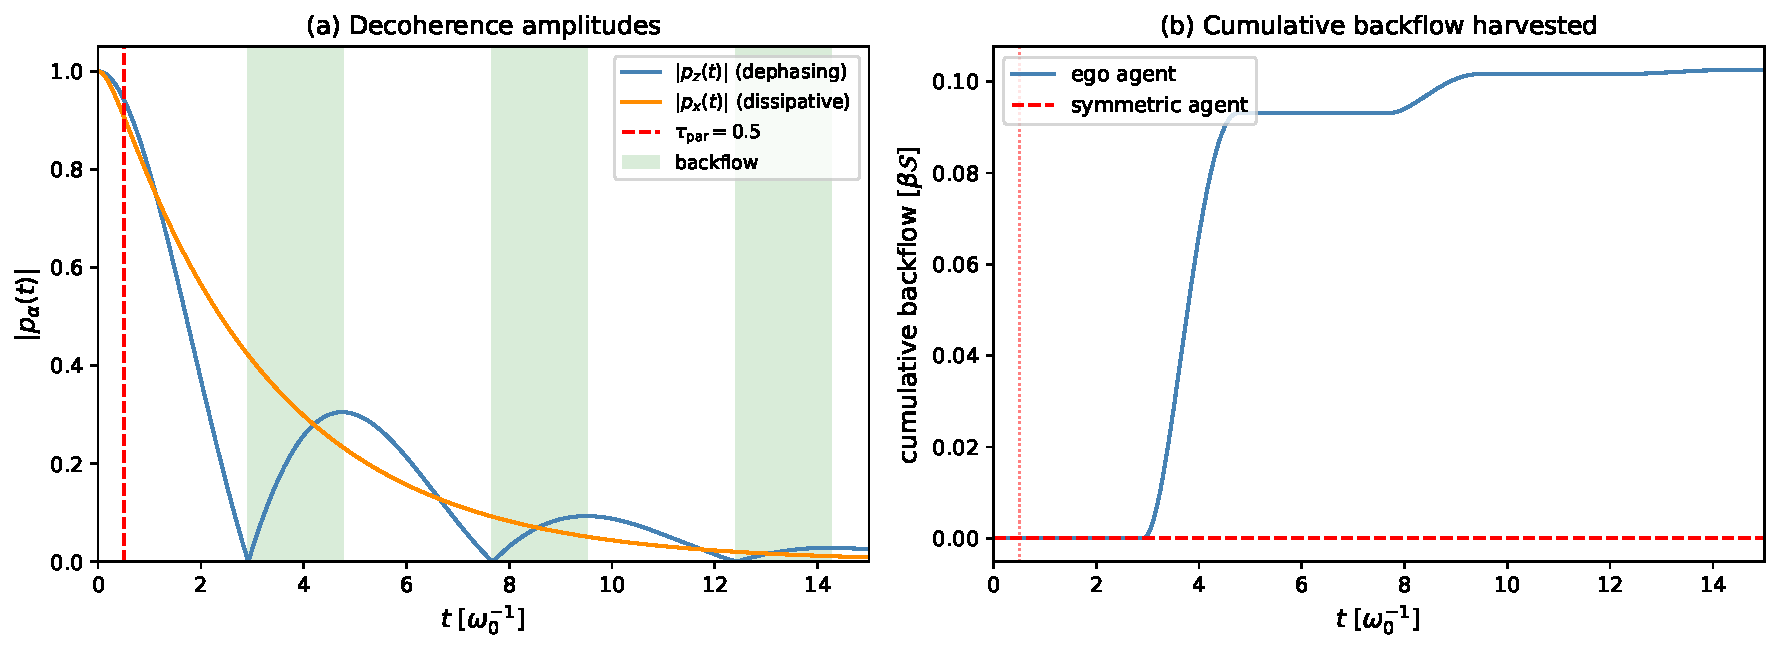
\includegraphics[width=\textwidth]{fig_ego.pdf}
\caption{%
Two-channel qubit model (Section~\ref{sec:example}) with
Lorentz--Drude spectral density.
\textbf{Parameters:}
$\omega_0 = 1$ (energy unit);
$\lambda_z = 1$, $\gamma_z = 0.5$ (dephasing, non-Markovian);
$\lambda_x = 0.3$, $\gamma_x = 5.0$ (dissipative,
$\sim$Markovian);
$\mathcal{C}_{\mathrm{budget}} = 2\,h_\mu$.
\textbf{Units:} time in $\omega_0^{-1}$.
\textbf{Regime:} low temperature ($\beta\omega_0 \gg 1$);
using the standard $T \to 0$ analytic
expression~\eqref{eq:decoherence_II}~%
\cite{BreuerPetruccione2002}.
\textbf{(a)}~Decoherence amplitudes $|p_z(t)|$ (blue,
non-Markovian, with backflow in green bands) and
$|p_x(t)|$ (orange, monotonic decay).
Red dashed: raw full-sweep depth $\tau_{\max} = 0.5$.
\textbf{(b)}~Cumulative backflow harvested.
Blue: ego agent (broken $\to \sigma_z$) exploits all three
revival intervals.
Red dashed: the stipulated raw full-sweep agent stops at
$\tau_{\max}$; all plotted backflow occurs later.
The growing gap is the \emph{ego dividend}.}
\label{fig:ego}
\end{figure}

\paragraph{Accounting check.}
The raw update load is $h_\mu D=4h_\mu$ while the budget is
$2h_\mu$, so that declared representation does not fit.  The example
then \emph{chooses} the two-component dephasing frame ($k^*=2$); for
that choice,
$R_{\mathcal{F}} = 2\,h_\mu
= \mathcal{C}_{\mathrm{budget}}$.  Saturation is an example property,
not a general consequence of monotonic distortion.

% ------------------------------------------------------------
\subsection{The Pointer-State Connection}
\label{subsec:pointer}

In this example the chosen basis coincides with an einselection
(environment-induced superselection) basis of the dephasing
model~\cite{Zurek2009}.
The coordinate optimization can select pointer-aligned components when
the declared distortion assigns them the highest survival value per
bit.  This alignment is verified only within a concrete model and is not
generic rate-distortion theorem.

\begin{remark}[Decoherence as symmetry-breaking catalyst]
\label{rem:decoherence}
The environment does not \emph{force} a specific gauge fixing.  A
pointer-aligned frame is selected only if the declared distortion and
encoder class rank it above the alternatives.  The present example
chooses that ranking; it does not derive it from bounded computation.
\end{remark}

% ============================================================
\section{The Cost of Ego}
\label{sec:cost}

Coordinate selection reduces the declared raw load but can introduce a
blind subspace. A fixed reference frame is a \emph{static}
gauge choice in a \emph{dynamic} environment.
If the environment changes, the ego becomes progressively
maladaptive.

\paragraph{Drift layer.}
Environmental change can occur at multiple levels:
parameter drift ($\lambda_\alpha(t)$, $\gamma_\alpha(t)$),
spectral-density deformation ($J(\omega, t)$), or
full process-distribution shift ($P_t(X)$).
For analytical tractability, we model drift at the
\emph{spectral-density parameter level} throughout this
section.  No monotone extension to arbitrary distribution shift is
claimed.

% ------------------------------------------------------------
\subsection{The Rigidity Trap}
\label{subsec:rigidity}

\begin{proposition}[Frame Rigidity under Drift]
\label{prop:rigidity}
Let the environment undergo slow drift: the spectral density
parameters change as
$\lambda_\alpha(t) = \lambda_\alpha^{(0)}
+ \varepsilon\,f_\alpha(t)$
for $\alpha \in \{z, x\}$, with drift rate
$\varepsilon > 0$.
Assume the supplied distortion has a locally unique $C^1$
minimizer $\mathcal{F}^*(\lambda)\in G$ and
$\lVert D_\lambda\mathcal F^*\rVert\leq K$ along the path.

If the agent's reference frame $\mathcal{F}$ is held fixed
(no recalibration), the mismatch between $\mathcal{F}$
and $\mathcal{F}^*(t)$ then obeys
\begin{equation}
\label{eq:mismatch}
\delta(t)
:= d_G\bigl(\mathcal{F},\, \mathcal{F}^*(t)\bigr)
\leq K\varepsilon \int_0^t \lVert\dot{f}(s)\rVert\,ds,
\end{equation}
where $d_G$ is the geodesic distance in the gauge group.
\end{proposition}

\begin{proof}
The chain rule and the stated sensitivity bound give
$\lVert\dot{\mathcal F}^*(t)\rVert
\leq K\varepsilon\lVert\dot f(t)\rVert$.
Integrating path length bounds the geodesic distance and yields
\eqref{eq:mismatch}.
\end{proof}

% ------------------------------------------------------------
\subsection{Stylized Drift Model}
\label{subsec:drift_model}

To quantify the loss of visibility of a fixed frame, we use the linear
drift supported by Proposition~\ref{prop:rigidity}.  No unstable
environmental dynamics or Lyapunov exponent is assumed.

\begin{definition}[Rotating optimal frame]
\label{def:drift}
Let the mismatch angle $\theta(t)$ between the agent's
fixed frame $\mathcal{F}$ and the instantaneous optimal
frame $\mathcal{F}^*(t)$ evolve as
\begin{equation}
\label{eq:theta}
\theta(t) = \theta_0+\varepsilon t,
\end{equation}
where $\theta_0 \in (0, \pi/4)$ is the initial misalignment
(so that the crossover time below is positive) and
$\varepsilon>0$ is the angular drift rate.  This is a local model up to
the first visibility crossover, not a claim about long-time motion on
the compact gauge group.

The visible and hidden survival components decompose
geometrically:
\begin{equation}
\label{eq:vis_hid_theta}
\mathcal{S}_{\mathrm{vis}}(t)
= \mathcal{S}_{\mathrm{tot}}\,\cos^2\theta(t),
\qquad
\mathcal{S}_{\mathrm{hid}}(t)
= \mathcal{S}_{\mathrm{tot}}\,\sin^2\theta(t),
\end{equation}
where $\mathcal{S}_{\mathrm{tot}}$ is the full survival
functional (invariant under frame rotation).
\end{definition}

% ------------------------------------------------------------
\subsection{The Prediction Error Divergence}
\label{subsec:divergence}

\begin{proposition}[Growth of the hidden component]
\label{prop:divergence}
Under the drift model~\eqref{eq:theta}--\eqref{eq:vis_hid_theta},
the hidden survival component grows as
\begin{equation}
\label{eq:divergence}
\bigl|\mathcal{S}_{\mathrm{hid}}(t)\bigr|
= |\mathcal{S}_{\mathrm{tot}}|\,\sin^2\!\bigl(\theta_0+
  \varepsilon t\bigr).
\end{equation}
For small angles ($\theta_0+\varepsilon t \ll 1$):
$|\mathcal{S}_{\mathrm{hid}}| \approx
|\mathcal{S}_{\mathrm{tot}}|(\theta_0+\varepsilon t)^2$.
\end{proposition}

\begin{proof}
Direct substitution of~\eqref{eq:theta}
into~\eqref{eq:vis_hid_theta}.
The small-angle expansion $\sin^2\theta\approx\theta^2$ gives the
quadratic form.
\end{proof}

% ------------------------------------------------------------
\subsection{Visibility Crossover and Conditional Gradient Reversal}
\label{subsec:delusion}

\begin{proposition}[Visibility crossover and a conditional gradient reversal]
\label{prop:delusion_model}
Under~\textup{(B1)--(B5)} with the drift
model~\eqref{eq:theta} and initial misalignment
$\theta_0 \in (0,\,\pi/4)$, an agent with a fixed
reference frame $\mathcal{F}$ reaches the visibility crossover
\begin{equation}
\label{eq:t_delusion}
t_{\mathrm{vis}}
= \frac{\pi/4-\theta_0}{\varepsilon},
\end{equation}
at which the hidden and visible magnitudes are equal.  For
$t>t_{\mathrm{vis}}$, the hidden magnitude is larger while
$\theta(t)<\pi/2$.  This geometric crossover alone implies neither
gradient anti-correlation nor failure of every in-frame detector.

There nevertheless exist specified controllers for which gradients do
reverse.  In the two-mode model
\begin{equation}
\label{eq:two_mode_losses}
\mathcal S_{\mathrm{vis}}(u)=-\tfrac12(u-1)^2,
\qquad
\mathcal S_{\mathrm{full}}(u,\theta)
=-\tfrac12\lVert u e_1-y^*(\theta)\rVert^2,
\quad
y^*(\theta)=\cos\theta\,e_1+\sin\theta\,e_2,
\end{equation}
the two scalar update directions are anti-correlated exactly when
\begin{enumerate}
\item[] $\cos\theta(t)<u<1$.
\end{enumerate}
Thus the reversal time is controller- and state-dependent; it need not
coincide with $t_{\mathrm{vis}}$.
\end{proposition}

\begin{proof}
The crossover $|\mathcal{S}_{\mathrm{hid}}|
= |\mathcal{S}_{\mathrm{vis}}|$ occurs when
$\sin^2\theta = \cos^2\theta$, i.e.,
$\theta(t_{\mathrm{vis}}) = \pi/4$.
Substituting~\eqref{eq:theta}:
$\theta_0+\varepsilon t_{\mathrm{vis}} = \pi/4$,
which gives~\eqref{eq:t_delusion}.
For~\eqref{eq:two_mode_losses},
$\partial_u\mathcal S_{\mathrm{vis}}=1-u$ and
$\partial_u\mathcal S_{\mathrm{full}}=\cos\theta-u$.
Their product is negative exactly when $u$ lies strictly between
$\cos\theta$ and $1$.  Outside that interval the two gradients agree
in sign or one vanishes.  The calculation exhibits the claimed effect
without promoting it to a universal consequence of visibility loss.
\end{proof}

\begin{remark}[Model scope]
\label{rem:linear_drift}
For $\theta_0=0$, the crossover occurs at
$t_{\mathrm{vis}} = \pi/(4\varepsilon)$.
With $\varepsilon = 0.01\,\omega_0$,
$t_{\mathrm{vis}} \approx 79\,\omega_0^{-1}$---long
enough for the agent to accumulate a false sense of
security, yet short on environmental timescales.
Neither this number nor the two-mode sign condition proves that an
agent cannot detect drift from residual statistics; Paper~III studies
one such detector.
\end{remark}

\begin{remark}[Why dithering does not help]
\label{rem:dithering}
One might ask whether the agent could escape the delusion
trap by randomly ``probing'' the background subspace
$V_{\mathrm{bg}}$---temporarily rotating its frame to
sample hidden components.
In the raw-coordinate model, a full probe competes with foreground
processing at the component-count rate in
Remark~\ref{rem:symmetry_tax}.  This does not prove dithering fails:
randomized exploration can reveal hidden directions, with a
model-dependent cost--benefit trade-off.  A deterministic in-frame
controller may lack a signal indicating when or where to probe.
As long as $|\mathcal{S}_{\mathrm{hid}}|
< |\mathcal{S}_{\mathrm{vis}}|$ (pre-delusion), the
in-frame performance metric $\mathcal{S}_{\mathrm{vis}}$
shows no anomaly.
The linear-drift visibility model below motivates monitoring residual
statistics, the subject of Paper~III, but does not rule out other
exploration policies.
\end{remark}

\begin{remark}[The ego as medicine and poison]
\label{rem:medicine_poison}
In this model, coordinate selection reduces raw load but creates a blind
subspace.  The visibility crossover below motivates Paper~III.  This is
a conditional engineering trade-off, not an irreversible logic chain.
\end{remark}

% ------------------------------------------------------------
\subsection{The Origin of Paper~III}
\label{subsec:paper3}

To respond to the visibility loss in this model, the agent may use a mechanism
to monitor the quality of its own reference frame---to
``observe its own observation.''
This requires a \emph{second-order control loop}: a
meta-controller that adjusts the gauge fixing $\sigma$ in
response to accumulated prediction errors.

The distribution of in-frame prediction residuals can itself change as
the frame becomes stale.  Paper~III studies whether a specified
likelihood model makes that change statistically identifiable.  This
paper does not prove that Fisher information is the unique detector or
that every controller must add such a loop.

This is the subject of Paper~III: the Fisher information
geometry of self-referential calibration, and the
thermodynamic cost of the loop that closes the chain
\emph{Chaos $\to$ Time $\to$ Self $\to$ Calibration}.

% ============================================================
\section{Numerical Demonstration}
\label{sec:numerical}

The preceding sections establish analytic bounds and a
worked example with a qubit in a two-channel bath.
We now compare budgeted coordinate-selection rules in a minimal
multi-dimensional system.  The observed attention concentration and
selection advantage are properties of this supplied algorithm and
environment.
Full code and parameters are provided for reproducibility.

% ------------------------------------------------------------
\subsection{Model}
\label{subsec:demo_model}

\paragraph{Environment.}
A $D$-dimensional linear prediction task with sparse
rotating support:
$y(t) = \mathbf{w}^*(t)^\top \mathbf{x}(t) + \xi(t)$,
$\mathbf{x}(t) \sim \mathcal{N}(\mathbf{0}, \mathbf{I}_D)$,
$\xi \sim \mathcal{N}(0, \sigma^2)$.
Only $m \ll D$ dimensions carry nonzero weight at any time;
the active support rotates every $\tau_{\mathrm{switch}}$
steps, modelling environmental drift.

\paragraph{Hard budget constraint.}
Per step, the agent may update only $k$ coordinates of its
weight vector (a hard processing budget), mirroring the
bounded computation assumption~(B2).

\paragraph{Agents.}
\begin{itemize}
\item \textbf{Budgeted selector}: selects the top-$k$
  dimensions by importance score---an exponential moving
  average of the signed per-coordinate gradient.  Signed
  accumulation ensures that noise dimensions (zero expected
  signal) cancel over time while signal dimensions persist,
  enabling reliable discrimination without access to the true
  support.
\item \textbf{Random-$k$ baseline}: selects $k$ dimensions
  uniformly at random each step.  This provides a
  budget-fair comparison with no persistent coordinate preference.
\end{itemize}

\noindent
The choice of \emph{signed} gradient EMA (rather than
squared-gradient magnitude) is structurally motivated:
for noise dimensions $\mathbb{E}[r\,x_i] = 0$, so the
signed accumulation cancels over time; for signal
dimensions $\mathbb{E}[r\,x_i] \neq 0$, so a consistent
directional bias persists.  The signed EMA thus acts as a
\emph{directional coherence filter} that discriminates
signal from noise without access to the true support---a
minimal model of a persistent coordinate preference.

\paragraph{Parameters.}
\begin{center}
\small
\begin{tabular}{@{}lcl@{}}
\toprule
\textbf{Quantity} & \textbf{Value} & \textbf{Role} \\
\midrule
$D$ & 64 & ambient dimension \\
$m$ & 8  & signal dimensions (sparse support) \\
$T$ & $10{,}000$ & horizon per trial \\
Seeds & 10 & independent replications \\
$\sigma$ & 0.3 & observation noise std \\
$\eta$ & 0.02 & SGD learning rate \\
$\lambda$ & 0.995 & weight decay per step \\
$k$ & 2, 4, 6, 8, 10, 12, 16, 20, 24, 32, 48, 64
  & budget grid \\
$\tau_{\mathrm{switch}}$ & $\{500, 1000, 2000\}$
  & support rotation period \\
\bottomrule
\end{tabular}
\end{center}

\paragraph{Attention entropy.}
Let $n_i$ be the number of updates coordinate $i$ receives
in a measurement window of the last $1{,}000$ steps.
The normalised update frequency
$p_i = n_i / \sum_j n_j$ defines the attention entropy:
\begin{equation}
\label{eq:H_attn}
H_{\mathrm{attn}} = -\sum_{i=1}^{D} p_i \ln p_i.
\end{equation}
Under uniform coordinate selection, $p_i = 1/D$ and
$H_{\mathrm{attn}} = \ln D$.  Under budget-constrained
selection, $H_{\mathrm{attn}}$ collapses away from $\ln D$,
measuring concentration of the update rule.  It is not by itself a
thermodynamic order parameter.

\paragraph{Oracle metric.}
Neither agent has access to $\mathbf{w}^*(t)$.
Performance is evaluated externally using the
weight-space mean-squared error
$\mathrm{MSE} = \|\hat{\mathbf{w}} - \mathbf{w}^*\|^2$,
averaged over post-burn-in steps.

% ------------------------------------------------------------
\subsection{Results}
\label{subsec:demo_results}

Figure~\ref{fig:kstar_scaling} shows the two key signatures.

\paragraph{Result 1: Attention entropy collapse
(Figure~\ref{fig:kstar_scaling}a).}
Under fixed support (no rotation), the attention entropy
$H_{\mathrm{attn}}$ exhibits a sharp collapse away from
$\ln D = \ln 64 \approx 4.16$ and increases monotonically
with $k$, consistent with a budget-induced concentration
of update mass onto signal-carrying dimensions.
For budgets near and below the signal scale ($k \leq m$),
$H_{\mathrm{attn}}$ remains $O(\ln m)$, consistent with
confinement to the signal subspace.
We use the collapse of $H_{\mathrm{attn}}$ away from
$\ln D$ as the order parameter of symmetry breaking;
a strict plateau at $\ln m$ is not expected under the
present re-selection dynamics and finite-window estimator.

\paragraph{Result 2: Selection advantage
(Figure~\ref{fig:kstar_scaling}b).}
Under rotating support, the mean-squared error gap
$\Delta\mathrm{MSE} = \mathrm{MSE}_{\mathrm{rnd}}
- \mathrm{MSE}_{\mathrm{sel}}$ is positive for
$k \lesssim 3m$ and peaks at tight budgets ($k = 2$)
where the selection advantage is strongest.
For $k \gg m$ the gap turns slightly negative
(the selector's commitment to stale dimensions costs
more than the random baseline's diversification),
before returning to zero at $k = D$.
The three $\tau_{\mathrm{switch}}$ curves are ordered:
slower drift (larger $\tau$) yields a larger peak gap,
with the ordering most visible at small $k$.

\begin{figure}[t]
\centering
\includegraphics[width=\textwidth]%
  {fig_paper2_kstar_scaling.pdf}
\caption{%
\textbf{Budgeted coordinate selection in the declared linear model.}
$D = 64$, $m = 8$, $T = 10{,}000$, 10 seeds, 95\% CI bands.
\textbf{(a)}~Attention entropy $H_{\mathrm{attn}}$ vs
budget $k$ (fixed support).  The empirical curve (blue)
collapses from $\ln D \approx 4.16$ toward an
$O(\ln m)$ floor as budget tightens.
For $k \leq m$, $H_{\mathrm{attn}}$ remains below
$\ln m \approx 2.08$ (green dashed), consistent with
confinement to the signal subspace.
\textbf{(b)}~Selection advantage
$\Delta\mathrm{MSE} = \mathrm{MSE}_{\mathrm{rnd}}
- \mathrm{MSE}_{\mathrm{sel}}$ vs budget $k$ under
rotating support.  The gap is positive for $k \lesssim 3m$
(selection helps), turns slightly negative at large $k$
(commitment cost exceeds diversification), and returns
to zero at $k = D$.  Slower drift ($\tau = 2000$)
yields a larger peak advantage.}
\label{fig:kstar_scaling}
\end{figure}

% ------------------------------------------------------------
\subsection{Scope of This Demonstration}
\label{subsec:demo_scope}

These simulations compare two supplied coordinate-selection rules in
the stated sparse linear model.  They do not establish a universal
symmetry-breaking transition or identify the capacity $k_{\max}$ with
an information-bottleneck optimum.

\medskip
This demonstration \textbf{does} show:
\begin{enumerate}
\item Under hard budget constraints, attention entropy
  collapses sharply away from $\ln D$ and remains
  $O(\ln m)$ for $k \leq m$---the agent confines its
  updates to the signal subspace.
  This measures concentration of the chosen update rule.
\item A budgeted selector that exploits importance-weighted
  selection systematically outperforms a budget-fair
  random baseline, consistent with a survival advantage
  for the parameter range shown.
\item The advantage scales with both budget tightness
  (smaller $k$) and environmental stability (larger
  $\tau_{\mathrm{switch}}$).
\end{enumerate}

\noindent
In summary, this demonstration establishes a model-specific selection
advantage and a measurable attention-concentration statistic; it does
not derive selection from the budget or claim universality across
architectures or environment classes.

\medskip
This demonstration does \textbf{not} show:
\begin{enumerate}
\item That $H_{\mathrm{attn}}$ reaches a strict plateau
  at $\ln m$ for all $k \leq m$.  Under the adaptive
  re-selection dynamics used here, the selector cycles
  within the signal subspace, producing
  $H_{\mathrm{attn}}$ values near but not locked to
  $\ln m$.  The relevant signature is the collapse
  \emph{away from} $\ln D$, not convergence to a
  specific lower bound.
\item That the specific form of the importance score
  (signed gradient EMA) is optimal.  It is one
  realisation of the selection mechanism.
\item That the results generalise to all environment
  classes.  The model uses Gaussian features, linear
  regression, and sparse rotating support.
\item That the delusion--correction cycle is addressed.
  This is the subject of Paper~III.
\item That a sharp thermodynamic phase transition occurs, or that
  $k=k_{\max}$ is the distortion-minimizing retained dimension.
\end{enumerate}

\paragraph{Reproducibility.}
\begin{sloppypar}
The complete simulation is a self-contained Python script
(\texttt{paper2\_kstar\_scaling\_demo.py}, ${\sim}\,540$
lines, requiring only NumPy and Matplotlib) with fixed
random seeds.  All figures in this section can be
reproduced by executing the script.  The following files
are included in the supplementary archive:
\begin{itemize}
\item \texttt{paper2\_kstar\_scaling\_demo.py} --- simulation script
\item \texttt{fig\_paper2\_kstar\_scaling.pdf} --- Figure~\ref{fig:kstar_scaling}
\item \texttt{kstar\_scaling\_data.csv} --- raw performance gap data
\end{itemize}
\end{sloppypar}

% ============================================================
\section{Discussion}
\label{sec:discussion}

% ------------------------------------------------------------
\subsection{Summary of Results}
\label{subsec:summary}

\begin{center}
\small
\setlength{\tabcolsep}{4pt}%
\begin{tabular}{@{}lP{6cm}c@{}}
\toprule
\textbf{Result} & \textbf{Statement} & \textbf{Sec.} \\
\midrule
Raw-channel load
  & A declared $D$-channel archive costs $D h_\mu$ per
    incremental update; this is accounting, not a lower bound
  & \ref{sec:ceiling} \\[3pt]
Compression existence
  & A minimizer exists in the supplied compact encoder class and has
    $k_{\mathrm{opt}}\leq k_{\max}$
  & \ref{subsec:RD_bound} \\[3pt]
Conditional frame selection
  & A chosen proper projection breaks the declared model symmetry when
    no invariant feasible encoder meets the target
  & \ref{subsec:SSB} \\[3pt]
Four diagnostics
  & Frame-dependent models can be audited using $\mathcal{B}_{\mathrm{select}}$,
    $\mathcal{B}_{\mathrm{frame}}$,
    $\mathcal{B}_{\mathrm{center}}$,
    $\mathcal{B}_{\mathrm{inc}}$
  & \ref{subsec:bias} \\[3pt]
Survival Decomposition
  & $\mathcal{S} = \mathcal{S}_{\mathrm{vis}} +
    \mathcal{S}_{\mathrm{hid}}$
  & \ref{subsec:effective} \\[3pt]
Uniform-channel trade-off
  & Predictive loss is approximately $1-k^*/D$ only under the
    uniform raw-channel assumption
  & \ref{subsec:tradeoff} \\[3pt]
Visibility crossover
  & Linear drift gives $t_{\mathrm{vis}}=(\pi/4-\theta_0)/\varepsilon$;
    gradient reversal requires a separate controller condition
  & \ref{subsec:delusion} \\[3pt]
Numerical demo
  & Attention concentration and model-specific selection advantage
    (Fig.~\ref{fig:kstar_scaling})
  & \ref{sec:numerical} \\
\bottomrule
\end{tabular}
\end{center}

% ------------------------------------------------------------
\subsection{Testable Predictions}
\label{subsec:predictions}

The conditional model claims can be tested without treating them as
universal laws.  First, vary $k$, $D$, and the support-switching time in
the declared sparse linear environment and compare the supplied selector
with random and alternative compressed baselines.  A sharp transition is
not predicted without a separately defined thermodynamic limit.

Second, estimate
$I(X_{\mathrm{past}};X_{\mathrm{future}})$ and
$I(\hat X_{\mathrm{past}};X_{\mathrm{future}})$ while varying $k/D$.
Linear $1-k/D$ scaling tests the uniform-allocation assumption in
Theorem~\ref{thm:tradeoff}; systematic curvature falsifies that
assumption rather than information theory.

Third, in a controlled rotating-feature task, measure both the visibility
ratio and the inner product of surrogate and oracle gradients.  The
linear model predicts the visibility crossover at
$t_{\mathrm{vis}}=(\pi/4-\theta_0)/\varepsilon$.  Proposition~\ref{prop:delusion_model}
predicts gradient reversal only for controllers entering the region
$\cos\theta(t)<u(t)<1$; coincidence of the two events is not required.

% ------------------------------------------------------------
\subsection{What This Paper Does and Does Not Show}
\label{subsec:claims}

This paper \textbf{does} show:
\begin{enumerate}
\item A declared raw $D$-channel archive has the stated component-count
  load, and a minimizer exists in the supplied compact encoder class.
\item A proper coordinate projection privileges a frame; under additional
  feasibility assumptions this can be interpreted as operational symmetry
  breaking (Remark~\ref{rem:conditional_ssb}).
\item Definition~\ref{def:bias} supplies four model diagnostics, with the
  extra controller and task assumptions needed by each made explicit.
\item Linear frame drift produces a visibility crossover, while the
  two-mode model exhibits a separate, conditional gradient reversal
  (Proposition~\ref{prop:delusion_model}).
\item A minimal computational demonstration measures attention
  concentration and a selection advantage over a budget-fair random baseline
  (Section~\ref{sec:numerical},
  Figure~\ref{fig:kstar_scaling}).
\end{enumerate}

\medskip
This paper does \textbf{not} show:
\begin{enumerate}
\item That bounded computation uniquely determines a privileged basis,
  forces symmetry breaking, or makes the chosen frame survival-optimal.
\item That symmetry breaking is necessary or sufficient for persistence.
\item That the ``ego'' implies or requires consciousness,
  subjective experience, or phenomenal awareness.
  The term is used strictly in the control-theoretic sense.
\item That this framework constitutes a theory of
  consciousness. It is a theory of computational optimality
  under thermodynamic constraints.
\item That the four diagnostics exhaust self-reference or follow from
  gauge fixing alone.
\item That the coordinate capacity is a Shannon rate--distortion bound or
  is achievable by a specific physical implementation.
\item That visibility loss forces gradient reversal or is undetectable.
  Paper~III analyzes one conditional calibration model.
\item That the framework constitutes or implies a
  philosophical or metaphysical claim about the nature
  of selfhood.
\item That this framework applies to all possible physical
  systems. It applies to systems
  satisfying the declared channel, encoder, controller, and drift
  assumptions.
\item That the Clifford algebra is the only possible
  algebraic setting. It is supplied here as a model input; Q-RAIF does
  not uniquely derive it.
\end{enumerate}

% ============================================================
% REFERENCES
% ============================================================
\begin{thebibliography}{99}

\bibitem{Liu2026TDOME_I}
S.~Liu, \emph{Non-Markovian Memory and Temporal Accumulation: A Conditional Thermodynamic Analysis}, Zenodo (2026), DOI: 10.5281/zenodo.18574342.

\bibitem{BreuerPetruccione2002}
H.-P.~Breuer and F.~Petruccione,
\emph{The Theory of Open Quantum Systems},
Oxford University Press (2002).

\bibitem{CrutchfieldYoung1989}
J.~P.~Crutchfield and K.~Young,
\emph{Inferring statistical complexity},
Phys.\ Rev.\ Lett.\ \textbf{63}, 105 (1989).

\bibitem{ShaliziCrutchfield2001}
C.~R.~Shalizi and J.~P.~Crutchfield,
\emph{Computational mechanics: Pattern and prediction,
structure and simplicity},
J.\ Stat.\ Phys.\ \textbf{104}, 817 (2001).

\bibitem{BialekNemenmanTishby2001}
W.~Bialek, I.~Nemenman, and N.~Tishby,
\emph{Predictability, complexity, and learning},
Neural Computation \textbf{13}, 2409 (2001).

\bibitem{Shannon1959}
C.~E.~Shannon,
\emph{Coding theorems for a discrete source with a
fidelity criterion},
IRE Nat.\ Conv.\ Rec., Part~4, pp.~142--163 (1959).

\bibitem{CoverThomas2006}
T.~M.~Cover and J.~A.~Thomas,
\emph{Elements of Information Theory},
2nd ed., Wiley (2006).

\bibitem{Simon1955}
H.~A.~Simon,
\emph{A behavioral model of rational choice},
Quarterly J.\ of Economics \textbf{69}, 99 (1955).

\bibitem{Tishby2000}
N.~Tishby, F.~C.~Pereira, and W.~Bialek,
\emph{The information bottleneck method},
in Proc.\ 37th Allerton Conf.\ on Communication, Control,
and Computing (1999); arXiv:physics/0004057 (2000).

\bibitem{Sims2003}
C.~A.~Sims,
\emph{Implications of rational inattention},
J.\ Monetary Economics \textbf{50}, 665 (2003).

\bibitem{JohnsonLindenstrauss1984}
W.~B.~Johnson and J.~Lindenstrauss,
\emph{Extensions of Lipschitz mappings into a Hilbert space},
Contemp.\ Math.\ \textbf{26}, 189 (1984).

\bibitem{Landauer1961}
R.~Landauer,
\emph{Irreversibility and heat generation in the
computing process},
IBM J.\ Res.\ Dev.\ \textbf{5}, 183 (1961).

\bibitem{Bennett1982}
C.~H.~Bennett,
\emph{The thermodynamics of computation---a review},
Int.\ J.\ Theor.\ Phys.\ \textbf{21}, 905 (1982).

\bibitem{Zurek2009}
W.~H.~Zurek,
\emph{Quantum Darwinism},
Nature Physics \textbf{5}, 181 (2009).

\bibitem{RivasHuelgaPlenio2014}
\'{A}.~Rivas, S.~F.~Huelga, and M.~B.~Plenio,
\emph{Quantum non-Markovianity: characterization,
quantification and detection},
Rep.\ Prog.\ Phys.\ \textbf{77}, 094001 (2014).

\bibitem{Liu2026HAFF_A}
S.~Liu, \emph{Emergent Geometry from Coarse-Grained Observable Algebras: The Holographic Alaya-Field Framework}, Zenodo (2026), DOI: 10.5281/zenodo.18361706.

\bibitem{Liu2026HAFF_B}
S.~Liu, \emph{Accessibility, Stability, and Emergent Geometry: Conceptual Clarifications on the Holographic Alaya-Field Framework}, Zenodo (2026), DOI: 10.5281/zenodo.18367060.

\bibitem{Liu2026HAFF_G}
S.~Liu, \emph{Structural Limits of Unification: Accessibility, Incompleteness, and a Programme-Level Final-Cut Diagnosis}, Zenodo (2026), DOI: 10.5281/zenodo.18402907.

\bibitem{Liu2026QRAIF_A}
S.~Liu, \emph{A Clifford-Encoding Model for Lorentzian Metrics in Entropic Gravity Frameworks}, Zenodo (2026), DOI: 10.5281/zenodo.18525876.

\bibitem{Liu2026QRAIF_B}
S.~Liu, \emph{Thermodynamic Stability Constraints on the Operator Algebra of Persistent Open Quantum Subsystems}, Zenodo (2026), DOI: 10.5281/zenodo.18525890.

\bibitem{Liu2026QRAIF_C}
S.~Liu, \emph{Conditional Image-Level Closure in the Q-RAIF Framework}, Zenodo (2026), DOI: 10.5281/zenodo.18528934.

\bibitem{PooleOzairVanDenOord2019}
B.~Poole, S.~Ozair, A.~Van~Den~Oord, A.~Alemi, and G.~Tucker,
\emph{On variational bounds of mutual information},
Proc.\ ICML, PMLR \textbf{97}, 5171--5180 (2019).

\bibitem{MehtaSchwab2012}
P.~Mehta and D.~J.~Schwab,
\emph{Energetic costs of cellular computation},
Proc.\ Natl.\ Acad.\ Sci.\ USA \textbf{109}, 17978 (2012).

\bibitem{GovernTenWolde2014}
W.~P.~Govern and P.~R.~ten~Wolde,
\emph{Optimal resource allocation in cellular sensing systems},
Proc.\ Natl.\ Acad.\ Sci.\ USA \textbf{111}, 17486 (2014).

\end{thebibliography}

\end{document}
